\chapter{Ergebnisse}
    Innerhalb diese Kapitels geht es zunächst um die Vorbereitung der Proben.
    Weiter geht es um den Umgang mit dem dreidimensionalen Datensatz sowie dessen Bearbeitung.
    Die verschiedenen extrahierten Darstellungen werden dann aufgenommen und analysiert.
    In dieser Arbeit untersuchten Gold und Nickeloxid Proben wurden alle in dem Versuchsaufbau aus \autoref{sec:Versuchsaufbau} vorbereitet und vermessen.
    Dabei betrug die Photonenenergie immer \SI{21.22}{\electronvolt}.
    Die Eisenoxid Proben wurden an der NanoESCA Beamline am Synchrotron Elettra in Triest präperiert und charakterisiert \footnote{Näheres zu diesem Versuchsaufbau und der Behandlung der Daten kann in \cite{ma-DJ} gefunden werden.}.

    \section{Gold}
        \begin{figure}
            \centering
            \begin{subfigure}{0.48\textwidth}
                \centering
                \includegraphics[height=5cm]{Au/2021_06_08_002_Au(111)_75eV}
                \subcaption{}
                \label{fig:LEED_Au}
            \end{subfigure}
            \begin{subfigure}{0.48\textwidth}
                \centering
                \includegraphics[height=5cm]{Au+5A/021_Au(111)+5A(40)_16eV.png}
                \subcaption{}
                \label{fig:LEED_Au+5A}
            \end{subfigure}
            \caption{Das Beugungsbild der sauberen Gold (111)-Oberfläche bei einer Elektronenenergie von \SI{75}{\electronvolt} \subref{fig:LEED_Au}.
            Und in \subref{fig:LEED_Au+5A} das LEED-Bild für die Kalibrierung des Pentacene bei einer Energie von \SI{16}{\electronvolt}.}
        \label{fig:Substrate}
        \end{figure}
        Zunächst geht es hier um das Substrat auf dem später der antiferromagnetische Nickeloxidfilm gewachsen wird.
        Das Substrat wurde zunächste mehrer Male durch ioneninduziertes Zerstäuben und anschließendes Aufheizen auf \SI{500}{\celsius} gereinigt.
        Es ergibt sich eine wohldefinierte Struktur der Oberfläche, was sich ebenfalls in dem Beugungsbild der niederenergetischen Elektronen in \autoref{fig:LEED_Au} erkennen lässt.
        Ferner sind scharfe Spots zu erkennen, ebenso wie die charakteristische kleineren Spots um die Hauptspots, die von der Fischgräten-Rekonstruktion herrühren.
        Die unterschiedlichen Intensität der einzelnen Reflexe rühren ebenfalls von der Rekonstruktion her.

        Um die Monolage an Molekülen, genauer dem Pentacene zu kalibrieren wird ebenfalls das Gold Substrat genutzt.
        Diese ordnen sich auf der Oberfläche an und ergeben das Beugungsbild in \autoref{fig:LEED_Au+5A}.
        Somit ist für die späteren Substrate ebenfalls die Molekülbedeckung evaluiert.

        \begin{figure}
            \centering
            \begin{subfigure}[t]{0.34\textwidth}
                \centering
                \includegraphics[height=4cm]{Au/BZ_Au.png}
                \subcaption{}
                \label{fig:BZ_Au}
            \end{subfigure}
            \begin{subfigure}[t]{0.62\textwidth}
                \centering
                \includegraphics[height=4cm]{Au/Band_Au111.png}
                \subcaption{}
                \label{fig:Band_Au}
            \end{subfigure}
            \caption{Die gemessene Winkelverteilung von Gold (111) an der Fermifläche \subref{fig:BZ_Au}.
            Eingezeichnet in rot ist die erste Brillouinzone und drei Hochsymmetriepunkte.
            In \subref{fig:Band_Au} ist die gemessene Bandstruktur von Gold (111) aufgetragen, welche sich durch Schneiden des dreidimensionale Datensatz entlang der orange gestrichelte Linien ergibt.}
        \end{figure}
        Die Eigenschaft, dass Gold einen Oberflächenzustand besitzt ist nützlich um festzustellen ob es sich um eine gut präperierte Oberfläche handelt.
        Der Oberflächenzustand lässt sich in \autoref{fig:BZ_Au} klar erkennen.
        Zusätzlich ist die erste Brillouinzone eingetragen sowie einige Hochsymmetriepunkte.
        Durch Schneiden entlang der orange gestrichelten Linien zwischen den Hochsymmetriepunkten ergibt sich die Bandstruktur, welche in \autoref{fig:Band_Au} dargestellt ist.
        % So lassen sich dann auch die Merkmale in dem integrierten Spektrum aus \autoref{fig:EDC_Au+5A} für das Gold indetifizieren.
        Direkt an der Oberfläche und nahe dem $\overline{\Gamma}$-Punkt befindet sich der Oberflächenzustand.
        Von der Fermikante bis hin zu etwa \SI{3.2}{\electronvolt} erstreckt sich parabelförmig das s-Band des Gold.
        Im Bereich zwischen \SIrange{2}{6.2}{\electronvolt} befinden sich die fünf d-Bänder, welche durch ihre flache Form und damit der Lokalisierung auffallen.

        \begin{figure}
            \centering
            \includegraphics[width=0.5\textwidth]{Au/Fermi_Au.png}
            \caption{Die integrierten Spektren an der Fermikante gemeinsam mit dem durchgeführtem Fit dessen für das Gold.}
            \label{fig:Fermi_Au}
        \end{figure}
        Die Bindungsenergie wurde ermittelt in dem die Photonenenergie von \SI{21.22}{\electronvolt} angenommen wurde und die Fermikante des Goldes bei \SI{16.55}{\electronvolt} in dem winkelintegrierten Spektrum aus \autoref{fig:Fermi_Au} gefittet wurde.
        Damit wird die Austrittsarbeit des Analysators zu \SI{4.72}{\electronvolt} bestimmt, nur dies fließt dann noch in die Gleichung \ref{eqn:Photoeffekt} ein.
        Dies ist vorallem für spätere messungen des Nickeloxidfilms wichtig, da es sich hierbei um einen Isolator handelt und somit die Fermienergie in den Bandlücke liegt.
        Wird die gesamte Länge des Spektrums betrachtet, also der Energieunterschied zwischen Fermikante und Ende des Sekundärelektronen, so lässt sich die Austrittsarbeit der Probe bestimmen.
        Für Gold lässt sich die Austrittsarbeit auf \SI{5.46}{\electronvolt} ermitteln, was das genau dem Literaturwerte entspricht~\cite{5A_4}.
        % Durch die Verschiebung des Abschnitt der Sekundärelektronen nach aufbringen des Pentacene ändert sich die Austrittsarbeit zu \SI{4.62}{\electronvolt}, was dabei sehr nah am Literaturwert von \SI{4.63}{\electronvolt} liegt~\cite{5A_4}.
        % Die Austrittsarbeit verschiebt sich also um \SI{0.84}{\electronvolt}, was auf ein starkes Oberflächendipolmoment hindeutet~\cite{5A_3}.
        % Auf Grund der Abwesenheit eines permaneten Dipols in den Molekülen und der Physisorption kann dies auf den Push-back Effekt zurück geführt werden.

        
    \section{Nickeloxid}    
        \begin{figure}
            \centering
            \includegraphics[height=5cm]{NiO/2021_06_15_019_NiO(111)_73eV_Thicklayer}
            \caption{Der Nickeloxidfilm (111) bei einer Elektronenenergie von \SI{73}{\electronvolt}.}
            \label{fig:LEED_NiO}
        \end{figure}
        Auf die saubere Goldprobe wird bei Raumtemperatur ein Nickeloxidfilm aufgebracht.
        Dies geschieht durch das Aufdampfen von Nickel mit einer Rate von \SI{0.3}{\angstrom\per\minute} in einer Sauerstoffatmosphäre von \SI{2e-6}{\milli\bar}.
        Es ergibt sich dabei das LEED Bild in \autoref{fig:LEED_NiO}.
        Im Vergleich zu den klaren und scharfen Spots des sauberen Gold scheinen diese etwas ausgewaschen zu sein.
        Die Ursache daran liegt in der nicht ganz perfekten Oberflächenbeschaffenheit \cite{NiO_34}.
        Durch die polare Oberflächennatur der (111)-Orientierung und der damit verbundenen Instabilität können verschiedene Relaxationsprozesse auftreten \cite{NiO_36, NiO_35, NiO_34, NiO_27, NiO_10}.
        Die Positionen der Punkte hat sich bei dem Nickeloxidfilm im Vergleich zum Gold nicht wesentlich verändert, ihre Gitterkonstanten sind also nahezu gleich.
        Auch die Intensitäten der Reflexe beim Nickeloxid sind nun gleich groß für alle Punkte.
        Aus der gleichen Symmetrie der Spots und der Abwesenheit zusätzlicher Spots kann eine $\text{p}(2 \times 2)$ Rekonstruktion \cite{NiO_37} und Domänenbildung der (100)-Orientierung \cite{NiO_36} ausgeschlossen werden.
        Die hier wahrscheinlichste Stabilisierung der Oberfläche ist die \ce{OH-}-Terminierung mit der $\text{p}(1 \times 1)$-Rekonstruktion \cite{NiO_35}.
        Hierbei wird das Oberflächenpotential durch Reduzierung der Oberflächenladung verkleinert und die Oberfläche wird thermodynamisch stabil.

        \begin{figure}
            \centering
            \begin{subfigure}[t]{0.48\textwidth}
                \centering
                \includegraphics[height=5cm]{NiO/NiO_Filmdicke.png}
                \subcaption{}
                \label{fig:EDC_NiO}
            \end{subfigure}
            \begin{subfigure}[t]{0.48\textwidth}
                \centering
                \includegraphics[height=5cm]{NiO/WKF_thickness.png}
                \caption{}
                \label{fig:WKF_NiO}
            \end{subfigure}
            \caption{\subref{fig:EDC_NiO} Die integrierten Spektren für zwei verschiedene Schichtdicken von \ce{NiO}. Als Referenz dient das integrierte Spektrum von Gold. 
            \subref{fig:WKF_NiO} Die integrierten Spektren im Bereich der Sekundärelektronen für verschiedene Schichtdicken von \ce{NiO}.}
        \end{figure}
        Durch Variation der Aufdampfzeiten lassen sich verschiedene Schichtdicken von Nickeloxidfilmen herstellen.
        Für zwei ausgewählte Zeiten sind die winkelintegrierten Spektren des Valenzbandbereiches in \autoref{fig:EDC_NiO} gemeinsam mit dem Spektrum des Substrates dargestellt.
        Zu erkennen ist, dass mit zunehmender Schichtdicke die charakteristischen Merkmale des Substrates abnehmen.
        Dafür steigt das Signal, was vom Nickeloxid herrührt an.
        Erkennbar ist somit auch die Oberflächenemfindlichkeit, der verwendeten Methode, da tiefer Lagen nur noch gering zum Signal beitragen.
        Aus der Verschiebung des Punktes an dem die Sekundärelektronen aufhören lässt sich erkennen, dass sich die Austrittsarbeit vom Gold zu dickeren Filmen Nickeloxid zu kleineren Werten verschiebt.
        Dies ist auch in \autoref{fig:WKF_NiO} für verschiedene Aufdampfzeiten dargestellt. 
        Kleine Verschiebungen können durch unterschiedliche Aufdampfbedingungen erklärt werden, denn es ist bekannt das durch Variation der Parameter gezielt die Eigenschaften manipuliert werden können.
        Vom dünnen Nickeloxidfilm zum dickeren Nickeloxidfilm wechselt sie von \SI{4.25}{\electronvolt} zu \SI{3.90}{\electronvolt}.
        Dies liegt daran, dass Sauerstofffehlstellen als negative Defekte gelten und somit die Austrittsarbeit verringern~\cite{IF_3}. \textbf{Eiegnlich bindet NiO lieber zusätzlichen Sauerstoff ein, was einer Erhöhung der Austrittsarbeit entsprechen würde}
        Die Austrittsarbeit des dicken Nickeloxidfilms passt \textbf{oder passt nicht zu Quelle und Wert}.
        Für den dünnen Nickeloxidfilm liegt die Austrittsarbeit mit den Molekülen dann bei \SI{4.14}{\electronvolt}.

        \begin{figure}
            \centering
            \includegraphics[height=7cm]{NiO/EDC_NiO_thick+exp.png}
            \caption{Winkelintegriertes Spektrum des dicken Nickeloxidfilms (rot), gemeinsam mit den identifizierten Merkmalen (blau).
            Überlagert dargestellt (schwarz) ist das gemessene Spektrum von Marre und Neddermeyer \cite{NiO_7}.} 
            \label{fig:EDC_NiO_thick}
        \end{figure}
        In der \autoref{fig:EDC_NiO_thick} ist das Valenzbandspektrum des dicken Nickeloxidfilms aufgetragen.
        Ebenfalls sind die Zuordnungen des Ursprungs der Merkmale gekennzeichnet.
        Bei einem Vergleich zwischen der gemessenen Kurve und der von Marre und Neddermeyer fällt auf, dass es eine konstante Verschiebung gibt.
        Ursache könnte die Bestimmung der Fermikante sein, denn bei Nickeloxid handelt es sich ja um einen Isolator.

        \begin{figure}
            \centering
            \includegraphics[height=4cm]{NiO/Band_NiO.png}
            \caption{Die gemessene Bandstruktur des dicken Nickeloxidfilms.}
            \label{fig:Band_NiO}
        \end{figure}
        Auch für Nickeloxid lässt sich aus dem dreidimensionalen Datensatz der Winkel und Energie aufgelöst ist die Bandstruktur extrahieren.
        Diese ist in \autoref{fig:Band_NiO} dargestellt.

        \begin{figure}
            \centering
            \begin{subfigure}[t]{0.48\textwidth}
                \centering
                \includegraphics[height=5cm]{NiO+5A/NiO_thick_5A_new.png}
                \subcaption{}
                \label{fig:EDC_NiO+5A}
            \end{subfigure}
            \begin{subfigure}[t]{0.48\textwidth}
                \centering
                \includegraphics[height=5cm]{NiO+5A/NiO_thick_5A_KE12_7.png}
                \subcaption{} % Map für Pentacene auf dicken Nickeloxidfilm bei einer kinetischen Energie von \SI{7.5}{\electronvolt}. Also Bindungsenergie von \SI{3.85}{\electronvolt}.
                \label{fig:MOT_NiO+5A}
            \end{subfigure}
            \caption{Integriertes Spektrum des Valenzband Bereiches für reines Nickeloxid und mit einer Monolage Pentacene \subref{fig:EDC_NiO+5A}, sowie ein winkelaufgelöstes Bild bei einer Bindungsenergie von \SI{3.85}{\electronvolt} \subref{fig:MOT_NiO+5A}.}
        \end{figure}
        Das Aufdampfen von einer Monolage Pentacene brachte kein LEED-Bild mehr zu stande.
        Nach dem Aufdampfen wurde versucht LEED-Bilder aufzunehmen, es waren allerdings nur leichte Substratspots sichtbar.
        So lässt sich schlussfolgern, dass sich die Moleküle auf der Oberfläche nicht anordnen.
        Dabei zeigt der direkte Vergleich der integrierten Spektren in \autoref{fig:EDC_NiO+5A} des reinen Nickeloxid und das mit Pentacene drauf deutliche zusätzliche Spitzen.
        Die Abwesenheit sehr ausgeprägter Merkmale in den impulsaufgelösten Bildern bestätigt die Annahme, dass sich die Moleküle auf der Oberfläche nicht regelmäßig anordnen.
        Ferner überlappen dann die einzelnen Merkmale im Impulsraum, sodass ein ausgewaschenes Bild entsteht.
        Auch wenn sich in den integrierten Spektren in \autoref{fig:EDC_NiO} klar zeigt, dass sich bei einigen Energien die Intensität erhöht ist in den entsprechenden Bildern keine klare Zuordnung möglich.
        Ein Beispiel ist in \autoref{fig:MOT_NiO+5A} zu sehen, dieses Bild wurde gewählt da ein deutliches Signal im integrierten Spektrum zu erkennen ist und die entsprechende Energie nicht zu weit weg von der Fermikante liegt.
        % Tendenziell sollten entsprechend winkelaufgelöste Bilder den theoretischen Berechnungen wie in \autoref{fig:MOT_Au+5A} entsprechen, da Substrate gleiche Symmetrien aufweisen.
        \begin{itemize}
            \item WKF Shift für dicken
            \item NiO-Spektrum Peaks zuordnen
            \item linear ansteigender Untergrund bei Molekülen ? zu sehen in der Differenz
        \end{itemize}


    \section{Eisen}
        \begin{figure}
            \centering
            \includegraphics[width=0.5\textwidth]{Fe/Fe3p_Fe.png}
            \caption{XPS Spektrum des $\ce{Fe}_{3\text{p}}$ Übergang des reinen Eisens. Hier passt der Fit mit einem Voigt (+Tougaard) sehr gut! $h\nu = \SI{200}{\electronvolt}$ und Polarisation s.}
            \label{fig:XPSFe3p_Fe}
        \end{figure}
        \begin{figure}
            \centering
            \includegraphics[height=5cm]{pFe/2021_09_07_001_passivatedFe(100)_44eV.png}
            \caption{Passiviertes Eisen (100) bei einer Elektronenenergie von \SI{44}{\electronvolt}.}
            \label{fig:LEED_pFe}
        \end{figure}
        Bei der verwendeten Eisenprobe handelt es sich um einen dünnen Eisenfilm, der auf einem Magnesiumoxid Substrat gewachsen wurde.
        Die Probe wurde ebenfalls durch leichtes ioneninduziertes Zerstäuben und aufheizen auf \SI{600}{\celsius} gerreinigt.
        Die Reinheit der Probe lässt sich auch am Spektrum des $\ce{Fe}_{3\text{p}}$ Übergangs in \autoref{fig:XPSFe3p_Fe} erkennen.
        Das Signal bei \SI{52.83}{\electronvolt} lässt sich nach Abzug eines Pseudo-Tougaard Untergrund sehr gut mit einer Pseudo-Voigt Funktion approximieren.
        Entsprechend gab sich die Halbwertsbreite zu \SI{2.11}{\electronvolt}.
        Um Verunreinigungen des sehr reaktiven sauberen Eisens zu vermeiden, wird die Probe anschließend direkt passiviert.
        Dies geschieht in einer Sauerstoffatmosphäre von \SI{1.3e-7}{\milli\bar} für fünf Minuten, während die Probe bei \SI{550}{\celsius} gehalten wird.
        Die Probe wird dann nocheinmal kurz auf \SI{600}{\celsius} aufgeheizt.
        Nun wird auch dessen Oberflächenbeschaffenheit kontrolliert und entsprechendes LEED-Bild ist in \autoref{fig:LEED_pFe} zu sehen.
        Sie Spots sind scharf und zeigen auch die Geometrie der $\ce{Fe}-\text{p}(1 \times 1)\ce{O}$ Struktur.
        Die gesamten Spots sind dabei nicht zentrosymmetrisch, da die Probe verkippt ist, wodurch auch der (0,0)-Reflex zu sehen ist.

        Um ebefalls die kinetische Energie in die übliche Bindungsenergie umzurechnen muss die Austrittsrabeit des Analysators bestimmt werden.
        Dies ist nötig, da es sich bei den Eisenmonooxid um einen Isolator handelt und hier also die Fermikante nicht ermittelt werden kann.
        Aus der Anpassung an der Fermikante des Eisens lässt sich dessen Position auf \SI{59.5}{\electronvolt} bei einer Photonenenergie von \SI{64}{\electronvolt} bestimmen.
        Dadurch lässt sich für die spätere Umrechnung in die Bindungsenergie die Austrittsarbeit des Analysators bei NanoESCA auf \SI{4.5}{\electronvolt} festlegen.
        Anzumerken ist, dass die Genauigkeit dieser Annahme nicht exakt ist, da zusätzlich die Fermikante durch ein starkes Signal überlagert wird.
        Aus dem Abschnitt der Sekundärelektronen lässt sich ferner dann die Austrittsarbeit der Eisenprobe auf \SI{4.06}{\electronvolt} bestimmen.
        
        \begin{figure}
            \begin{subfigure}[t]{0.34\textwidth}
                \centering
                \includegraphics[height=4cm]{Fe/BZ_Fe.png}
                \subcaption{}
                % Die Brillouinzone des reinen Eisens bei einer Bindungsenergie von \SI{0.3}{\electronvolt}.
                % Eigezeichnet sind auch die Vektoren, sowie einige Hochsymmetrierichtungen.
                % Die Kantenlänge der BZ ist $\frac{2\pi}{a} = \SI[per-mode=reciprocal]{2.20}{\per\angstrom}$.
                % Im Zentrum liegt der $\overline{\Gamma}$-Punkt, der Abstand zum $\overline{X}$-Punkt ist $\frac{2\pi}{2 \cdot a} = \SI[per-mode=reciprocal]{1.10}{\per\angstrom}$ und zum $\overline{M}$-Punkt $\frac{2\pi}{2 \cdot a} \sqrt{2} = \SI[per-mode=reciprocal]{1.55}{\per\angstrom}$.
                % Verwendete Photonenenergie war \SI{64}{\electronvolt} und die Polarisation p.
                \label{fig:BZ_Fe}
            \end{subfigure}
            \begin{subfigure}[t]{0.62\textwidth}
                \centering
                \includegraphics[height=4cm]{Fe/Band_Fe.png}
                \subcaption{}
                % Die Bandstruktur des reinen Eisens entlang einiger Hochsymmetrierichtungen.
                % Verwendete Photonenenergie war \SI{64}{\electronvolt} und die Polarisation p.
                \label{fig:Band_Fe}
            \end{subfigure}
            \caption{\subref{fig:BZ_Fe} Die erste Oberflächenbrillouinzone des Eisen (gelb), gemeinsam mit den Hochsymmetriepunkten. Das Bild ist bei einer Bindungsenergie von \SI{0.3}{\electronvolt} aufgenommen.
            \subref{fig:Band_Fe} Die entlang der grünen Linien in \subref{fig:BZ_Fe} extrahierte Bandstruktur der Eisen (100)-Oberfläche für eine Photonenenergie von \SI{64}{\electronvolt}.}
        \end{figure}
        Wie schon für das Gold lässt sich auch die Oberflächenbrillouinzone des Eisens darstellen. 
        Dies ist in \autoref{fig:BZ_Fe} geschehen.
        Aus ihr lässt sich dann anschließend wieder die Bandstruktur extrahieren, welche in \autoref{fig:Band_Fe} abgebildet ist.
        

    \section{Magnetit}
        \begin{figure}
            \centering
            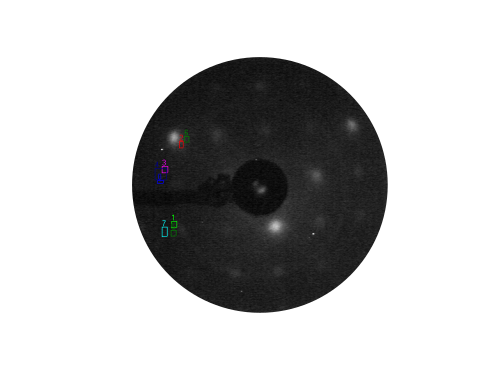
\includegraphics[height=5cm]{Fe3O4/2021_09_07_012_FeO(100)_44eV.png}
            \caption{\ce{Fe3O4} (100) bei einer Elektronenenergie von \SI{44}{\electronvolt}.}
            \label{fig:LEED_Fe3O4}
        \end{figure}
        Auf dem der passivierten Eisenoberfläche wird Eisen mit einer Rate von \SI{0.6}{\ML\per\minute} und einem Sauerstoffdruck von \SI{2e-7}{\milli\bar} aufgedampft.
        Dabei wird die Probe auf eine Temperatur von \SI{230}{\celsius} gehalten.
        Zum abschluss wird die Temperatur auf \SI{600}{\degree} für fünf Minuten erhöht.
        So ergibt sich in \autoref{fig:LEED_Fe3O4} das Beugungsbild der Oberfläche.
        Es sind klar deutlich mehr Spots zu erkennen, die auf eine $\text{p}(1 \times 1)$-Überstruktur hindeuten.

        \begin{figure}
            \centering
            \includegraphics[height=5cm]{Fe3O4/AES_Fe3O4.png}
            \caption{Das Augerspektrum der Magnetitprobe.}
            \label{fig:Auger_Fe3O4}
        \end{figure}
        Die Konzentrationen an Sauerstoff und Eisen werden mittels Augerelektronenspektroskopie analysiert.
        So ergibt sich das Augerspektrum in \autoref{fig:Auger_Fe3O4}.
        Hierbei kann das Signal bei \SI{503}{\electronvolt} dem KLL-Übergang des Sauerstoffs und dem Eisen die Signale bei \SI{598}{\electronvolt}, \SI{651}{\electronvolt} und \SI{703}{\electronvolt} für den LMM-Übergang zugeordnen werden. 
        Die drei unterschiedlichen Energien für das Eisen tauchen durch die Spin-Bahn-Aufspaltung des Eisens auf.
        Das Peakverhältnis zwischen dem Sauerstoffsignal bei \SI{503}{\electronvolt} und dem Signal für Eisen bei \SI{651}{\electronvolt} ergibt einen Wert von \num{3.14}~\cite{FeO_1, Auger}.
        Aus der Literatur ist bekannt das für Magnetit ein Wert von \num{3.86} erwartet wird~\cite{FeO_1}.
        Der ermittelte Wert weicht dabei nach unten ab, was durch das zusätzliche Aufheizen auf \SI{600}{\degree} erklärt werden kann.
        Dabei kommt es zur Umstrukturierung der Oberfläche und in Folge dessen auch zur Desorption von Sauerstoff.

        Wird das Verhältnis der Intensitäten der Signale bei \SI{503}{\electronvolt} und \SI{703}{\electronvolt} unter Beachtung der elementspezifischen Sensetivität ausgewärtet ergibt sich das stöchimetrischen Verhältnis.
        Die Sensetivität für Sauerstoff liegt bei \num{0.5} und die des Eisens bei \num{0.2} bei der Verwendung von \SI{3}{\kilo\electronvolt} Primärelektronen.
        Konzentration $c_i = \frac{I_i/S_i}{\sum_j I_j/S_j}$.
        Dies lässt sich hier auf $\ce{O}:\ce{Fe} = \num{0.55}:\num{0.45}$ bestimmen.
        Problem bereitet natürlich das Substrat, was ebenfalls aus Eisen besteht und auch die passivierte Schicht enthält bereits Sauerstoff.

        \begin{figure}
            \centering
            \includegraphics[height=5cm]{Fe3O4/Fermi_Fe3O4.png}
            \caption{Das Spektrum des Valenzbandes bei einer Photonenenergie von \SI{64}{\electronvolt} und der p Polarisation des \ce{Fe3O4}.}
            \label{fig:EDC_Fe3O4}
        \end{figure}
        Wird sich das Valenzband erneut genauer angeschaut so ergibt sich das winkelintegrierte Spektrum in \autoref{fig:EDC_Fe3O4}.
        Zusammen mit dem Ende der Sekundärelektronen ergibt sich die Austrittsarbeit dabei zu \SI{4.35}{\electronvolt}.

        \begin{figure}
            \centering
            \begin{subfigure}[t]{0.48\textwidth}
                \centering
                \includegraphics[height=5cm]{Fe3O4/O1s_Fe3O4.png}
                \subcaption{Spektrum des $\ce{O}_{1\text{s}}$ Übergang. Fit mit zwei Peaks (kleiner Shirley) sehr gut (einer O, der andere OH - Kontamination evtl vom Aufdampfen?).
                Verwendete Photonenenergie war \SI{650}{\electronvolt} und die Polarisation s.}
                \label{fig:XPSO1s_Fe3O4}
            \end{subfigure}
            \begin{subfigure}[t]{0.48\textwidth}
                \centering
                \includegraphics[height=5cm]{Fe3O4/Fe3p_Fe3O4.png}
                \subcaption{Spektrum des $\ce{Fe}_{3\text{p}}$ Übergang. Gleiches Problem wie beim \ce{FeO} (s. \autoref{fig:XPSFe3p_Fe}) funktioniert abenfalls besser mit Tougaard als Shirley.
                Verwendete Photonenenergie war \SI{200}{\electronvolt} und die Polarisation s.}
                \label{fig:XPSFe3p_Fe3O4}
            \end{subfigure}
            \caption{Die XPS Spektren der Kernniveaus für das Magnetit.}
            \label{fig:XPS_Fe3O4}
        \end{figure}
        Um genauer zu überprüfen wird auch die chemisch sensetive Methode der Röntgenphotoelektronenspektroskopie angewendet.
        Die entsprechenden Spektren des $\ce{O}_{1\text{s}}$ Signals, sowie des $\ce{Fe}_{3\text{p}}$ Signals sind in \autoref{fig:XPS_Fe3O4} dargstellt.

        Wie bereits schon bei dem Nickeloxid brachte das Aufdampfen von einer Monolage Pentacene keine geordnete Struktur mit sich.


    \section{Wüstit}
        \begin{figure}
            \centering
            \includegraphics[height=5cm]{FeO/2021_09_09_004_FeO_44eV.png}
            \caption{\ce{FeO} (100) bei einer Elektronenenergie von \SI{44}{\electronvolt}.}
            \label{fig:LEED_FeO}
        \end{figure}
        Um die Wüstitstruktur zu erhalten wird die Magnetitstruktur zunächst auf \SI{650}{\celsius} aufgeheizt.
        Anschließend werden vermehrt Sauerstoffatome durch ioneninduziertes Zerstäuben ausgelöst um so die Wüstit Zusammensetzung zu erhalten.
        Im Anschluss wird die Probe nochmal auf \SI{650}{\celsius} erwärmt um die Fehlstellen auszuheilen.
        Durch die induzierte Umordnung der Atome ergibt sich dann die gewünschte Struktur, welche in dem LEED Bild aus \autoref{fig:LEED_FeO} zu erkennen ist.
        Die Intensitäten sind beim Eisenoxid im Gegensatz zu dem passivierten Eisen invertiert, wobei die zuvor starken Spots nicht mehr sichtbar sind.
        Trotz der gleichen Elektronenenergie von \SI{125}{\electronvolt} sind die Spots leicht nach außen gewandert.
        Dies Widerspricht sich mit der eigentlich größeren Gitterkonstante von Eisenoxid im Bezug auf die $\text{p}(1 \times 1)\ce{O}$ Überstruktur des passivierten Eisens.
        Was dennoch auffällig ist, sind die nicht mehr präsenten zusätzlichen Punkte durch die Überstruktur wie beim \ce{Fe3O4} in \autoref{fig:LEED_Fe3O4}.

        \begin{figure}
            \centering
            \includegraphics[height=5cm]{FeO/AES_FeO.png}
            \caption{Das Augerspektrum der Wüstitprobe.}
            \label{fig:Auger_FeO}
        \end{figure}
        \begin{figure}
            \centering
            \begin{subfigure}[t]{0.48\textwidth}
                \centering
                \includegraphics[height=5cm]{FeO/O1s_FeO.png}
                \subcaption{Spektrum des $\ce{O}_{1\text{s}}$ Übergang. Fit mit einem Peak (kleiner Shirley) sehr gut.
                Verwendete Photonenenergie war \SI{650}{\electronvolt} und die Polarisation s.}
                \label{fig:XPSO1s_FeO}
            \end{subfigure}
            \begin{subfigure}[t]{0.48\textwidth}
                \centering
                \includegraphics[height=5cm]{FeO/Fe3p_FeO.png}
                \subcaption{Spektrum des $\ce{Fe}_{3\text{p}}$ Übergang. Zuornung sehr schwierig, ein großer Peak bei kleinen BE und ein kleiner bei großen BE passen. Aber auch zwei etwa gleichgroße Peaks. Je nach dem wie die Parameter gewählt und festgestzt werden.
                Verwendete Photonenenergie war \SI{200}{\electronvolt} und die Polarisation s.}
                \label{fig:XPSFe3p_FeO}
            \end{subfigure}
            \caption{}
            \label{fig:XPS_FeO}
        \end{figure}
        Das Verhältnis aus Sauerstoff und Eisen kann dabei erneut mittels Augerelektronenspektroskopie überprüft werden.
        Auch das Augerspektrum in \autoref{fig:Auger_FeO} mit dem bereits von Carpa u.A. \cite{FeO_1} entdecken Augerelektronenspektrum für Eisenoxid zeigt gute Übereinstimmung.
        Ebenfalls deutet das Peakverhältnis von dem Sauerstoffsignal und Eisen mit \num{2.68} auf $\ce{FeO}$ hin, da dies nur leicht unterhalb des Wertes aus der Literatur von \num{2.89} liegt \cite{FeO_1}.
        Einen genaueren Einblick welche Struktur vorliegt kann erneut die Röntgenphotoelektronenspektroskopie bieten.
        Die entsprechenden Spektren sind in \autoref{fig:XPS_FeO} zu finden.

        % \begin{figure}
        %     \centering
        %     \includegraphics[width=0.5\textwidth]{FeO/Fermi_FeO.png}
        %     \caption{Valenzbandspektrum der des \ce{FeO} bei einer Photonenenergie von \SI{64}{\electronvolt}. Zusätzlich eingetragen ist der Fit des Beginns des Spektrums.}
        %     \label{fig:Fermi_FeO}
        % \end{figure}
        % Ebenso ist in \autoref{fig:Fermi_FeO} die Elektronendichtekurve für den Valenzbandbereich des \ce{FeO} aufgetragen.
        % Zusätzlich wurde der Beginn des Spektrums in der kinetischen Energie auf \SI{58.93}{\electronvolt} bestimmt.
        % Der Beginn des Spektrums sieht einer Fermikante sehr ähnlich.
        \begin{figure}
            \centering
            \includegraphics[width=0.5\textwidth]{FeO/EDC_FeO.png}
            \caption{Valenzbandspektrum der des \ce{FeO} bei einer Photonenenergie von \SI{64}{\electronvolt}. Blau gestrichelt sind die identifizierten Merkmale, die das Spektrum bestimmen.}
            \label{fig:EDC_FeO}
        \end{figure}
        Das Valenzbandspektrum in \autoref{fig:EDC_FeO} setzt sich aus maßgeblich vier Signalen zusammen bei den Energien \SI{1.5}{\electronvolt} (Fe3p \cite{Grenet et al. - 1980 - On the FeO valence band photoemission spectra.pdf}), \SI{4}{\electronvolt}, \SI{5.4}{\electronvolt} und \SI{6.2}{\electronvolt} (vermutlich O 2p).
        Aus dem Punkt an dem die Sekundärelektronen aufhören und der Fermikante lässt sich die Austrittsarbeit auf \SI{3.06}{\electronvolt} bestimmen.
        Durch das Aufdampfen der Moleküle verschiebt sich diese dann zu \SI{3.51}{\electronvolt}.

        \begin{figure}
            \begin{subfigure}[t]{0.34\textwidth}
                \centering
                \includegraphics[height=4cm]{FeO/BZ_FeO.png}
                \subcaption{}
                % Die Brillouinzone des Eisensoxid bei einer Bindungsenergie von \SI{1.95}{\electronvolt}.
                % Eigezeichnet sind auch die Vektoren, sowie einige Hochsymmetrierichtungen.
                % Die Kantenlänge der BZ ist $\frac{2\pi}{a}\sqrt{2} = \SI[per-mode=reciprocal]{2.89}{\per\angstrom}$.
                % Im Zentrum liegt der $\overline{\Gamma}$-Punkt, der Abstand zum $\overline{X}$-Punkt ist $\frac{2\pi}{2 \cdot a}\sqrt{2} = \SI[per-mode=reciprocal]{1.45}{\per\angstrom}$ und zum $\overline{M}$-Punkt $\frac{2\pi}{a} = \SI[per-mode=reciprocal]{2.05}{\per\angstrom}$ \cite{Hüfner}.
                % Verwendete Photonenenergie war \SI{64}{\electronvolt} und die Polarisation p.}
                \label{fig:BZ_FeO}
            \end{subfigure}
            \begin{subfigure}[t]{0.62\textwidth}
                \centering
                \includegraphics[height=4cm]{FeO/Band_FeO.png}
                \subcaption{}
                % Die Bandstruktur des Eisenmonooxid entlang einiger Hochsymmetrierichtungen.
                % Verwendete Photonenenergie war \SI{64}{\electronvolt} und die Polarisation p.
                \label{fig:Band_FeO}
            \end{subfigure}
            \caption{Die Oberflächenbrillouinzone des Eisenmonooxid bei einer Bindungsenergie von \SI{1.95}{\electronvolt} \subref{fig:BZ_FeO}.
            Die entlang der grünen Linien aus \subref{fig:BZ_FeO} extrahierte Bandstruktur bei $h\nu = \SI{64}{\electronvolt}$ \subref{fig:Band_FeO}.}
        \end{figure}
        Auch für das Wüstit lässt sich die Oberflächenbrillouinzone definieren, die in \autoref{fig:BZ_FeO} abgebildet ist.
        Daraus lässt sich durch Schneiden des dreidimensionalen datensatzes die Bandstruktur gewinnen, welche in \autoref{fig:Band_FeO} zu sehen ist.

        \begin{figure}
            \centering
            \begin{subfigure}[t]{0.48\textwidth}
                \centering
                \includegraphics[height=5cm]{FeO/XMCD_FeO.png}
                \caption{Spektren für links- und rechtzirkular polarisiertes Licht und ihre Differenz dem XMCD Signal.}
                \label{fig:XMCD}
            \end{subfigure}
            \begin{subfigure}[t]{0.48\textwidth}
                \centering
                \includegraphics[height=5cm]{FeO/XMLD_FeO.png}
                \caption{Spektren für s- und p- polarisiertes Licht, sowie dessen Differenz dem XMLD Signal.}
                \label{fig:XMLD}
            \end{subfigure}
            \caption{Die verschiedenen XAS Messungen mit unterschiedlichen Polarisationen. Aus der Differenz ergeben sich dann die XMCD und XMLD Signale.}
            \label{fig:XAS_FeO}
        \end{figure}
        Mit Hilfe des magnetischen Röntgen-Zirkular-Dikorismus und magnetischen Röntgen-Linear-Dikorismus lassen sich die magnetischen Eigeschaften des Substrates untersuchen.
        Beide Spektren der Röntgenabsorptionsmessungen sind in \autoref{fig:XAS_FeO} zu sehen.
        
        \begin{figure}
            \centering
            \begin{subfigure}[t]{0.48\textwidth}
                \centering
                \includegraphics[height=3.7cm]{FeO+5A/FeO_5A_34_80eV.png}
                \subcaption{\SI{0.70}{\electronvolt}}
                % Das Bild für eine kinetische Energie von \SI{34.80}{\electronvolt}, also \SI{0.70}{\electronvolt} Bindungsenergie.
                \label{fig:MOT_FeO+5A_exp_1}
            \end{subfigure}
            \begin{subfigure}[t]{0.48\textwidth}
                \centering
                \includegraphics[height=3.7cm]{FeO+5A/MO_LUMO_RT_RT.png}
                \subcaption{LUMO}
                % Das LUMO mit Symmetrisierung zweier um \SI{90}{\degree} verdrehten Übergitter.
                \label{fig:MOT_FeO+5A_theo_1}
            \end{subfigure}
            \centering
            \begin{subfigure}[t]{0.48\textwidth}
                \centering
                \includegraphics[height=3.7cm]{FeO+5A/FeO_5A_33_75eV.png}
                \subcaption{\SI{1.75}{\electronvolt}}
                % Das Bild für eine kinetische Energie von \SI{33.75}{\electronvolt}, also \SI{1.75}{\electronvolt} Bindungsenergie.
                \label{fig:MOT_FeO+5A_exp_2}
            \end{subfigure}
            \begin{subfigure}[t]{0.48\textwidth}
                \centering
                \includegraphics[height=3.7cm]{FeO+5A/MO_HOMO_RT_RT.png}
                \subcaption{HOMO}
                % Das HOMO mit Symmetrisierung zweier um \SI{90}{\degree} verdrehten Übergitter.
                \label{fig:MOT_FeO+5A_theo_2}
            \end{subfigure}
            \centering
            \begin{subfigure}[t]{0.48\textwidth}
                \centering
                \includegraphics[height=3.7cm]{FeO+5A/FeO_5A_32_15eV.png}
                \subcaption{\SI{3.35}{\electronvolt}}
                % Das Bild für eine kinetische Energie von \SI{32.15}{\electronvolt}, also \SI{3.35}{\electronvolt} Bindungsenergie.
                \label{fig:MOT_FeO+5A_exp_3}
            \end{subfigure}
            \begin{subfigure}[t]{0.48\textwidth}
                \centering
                \includegraphics[height=3.7cm]{FeO+5A/MO_HOMO1_RT_RT.png}
                \subcaption{HOMO-1}
                % Das HOMO-1 mit Symmetrisierung zweier um \SI{90}{\degree} verdrehten Übergitter.
                \label{fig:MOT_FeO+5A_theo_3}
            \end{subfigure}
            \centering
            \begin{subfigure}[t]{0.48\textwidth}
                \centering
                \includegraphics[height=3.7cm]{FeO+5A/FeO_5A_30_95eV.png}
                \subcaption{\SI{4.55}{\electronvolt}}
                % Das Bild für eine kinetische Energie von \SI{30.95}{\electronvolt}, also \SI{4.55}{\electronvolt} Bindungsenergie.
                \label{fig:MOT_FeO+5A_exp_4}
            \end{subfigure}
            \begin{subfigure}[t]{0.48\textwidth}
                \centering
                \includegraphics[height=3.7cm]{FeO+5A/MO_HOMO2_RT_RT.png}
                \subcaption{HOMO-2}
                % Das HOMO-2 mit Symmetrisierung zweier um \SI{90}{\degree} verdrehten Übergitter.
                \label{fig:MOT_FeO+5A_theo_4}
            \end{subfigure}
            \caption{Vergleich der gemessenen Intensitätsverteilung für verschiedene Bindungsenergien mit den theoretisch berechneten Intensitätsverteilungen.}
            \label{fig:MOT_FeO_5A}
        \end{figure}
        Das Aufdampfen wie einer Monolage Pentacene brachte erneut kein homogenes und von einer geordneten Struktur herrührendes LEED-Bild zustande.
        Im Widerspruch zu dem nicht Vorhandensein entsprechnder Beugungsreflexe und damit sich die Moleküle nicht auf der Oberfläche ordnen sind in den Tomographiebildern Merkmale von Molekülen zu erkennen.
        Diese Merkmale können sich nur ausbilden, wenn sich die Moleküle regelmäßig und in gleicher Orientierung anordnen.
        Anderenfalls würden sich die Photoemissionströme überlagern und es gäbe verschwommene Bilder.
        Einige Zuordnungen sind in \autoref{fig:MOT_FeO_5A} zu finden.
        Die theoretisch berechneten Bilder wurden mit Hilfe des Python Programms \textit{kmap.py} erstellt~\cite{brandstetter_kmappy_2021}.
        Anschließend wurden die Symmetrien berücksichtigt, in dem zwei um \SI{90}{\degree} zueinander verdrehten Bilder aufsummiert wurden.

        \begin{figure}
            \centering
            \includegraphics[height=5cm]{pFe/Photonenenergie.png}
            \caption{Vergleich des VB-Spektrums bei \SI{64}{\electronvolt} und \SI{40}{\electronvolt} Photonenenergie des passivierten Eisens.}
            \label{fig:Photonenenergie}
        \end{figure}
        Allerdings ist die eindeutige Zuordnung recht schwierig, da eine Referenzmessung des Substrates bei entsprechnder Photonenenergie nicht aufgenommen wurde.
        Bei einer anderen Photonenenergie aufgenommene Spektren lassen sich nur schwer als Vergleich heranziehen, da diese deutliche Unterschiede aufweisen können.
        Als Bespiel sind hier in \autoref{fig:Photonenenergie} zwei Spektren des passivierten Eisens dargestellt bei unterschiedlicher Photonenenergie.
        Klar zu erkennen ist schon der Unterschied in der Gesamtintensität, was durch den unterschiedlichen Photonenfluss der Beamline für verschiedene Energien zustande kommt.
        Aber auch bei der betrachtung der winkelaufgelösten Bilder sind klare Unterschiede hinsichtlich der Merkmale erkennbar.
        Teilweise zeigen die Bilder bei den gleichen Energien wie die HOMO bis HOMO-2 Orbitale sehr ähnliche Signale wie mit den Molekülen.

        Es kann davon ausgegangen werden, dass es sich bei der Wechselwirkung um die Chemisorption handelt, denn auch das LUMO wird besetzt.
        Um dies zu erlangen muss vorher Ladung zwischen dem Molekülen und dem Substrat ausgetauscht worden sein, was das Merkmal der Chemisorption ist.

  
    \section{NOTIZEN}
    \subsection{datendeutung}
        \begin{itemize}
            \item Zuordnung des Fe3p Peaks schwer. Manche sagen sechs Peaks voraus \cite{FeO_14, FeO_17, FeO_15} wegen der Finestruktur, andere zwei (Fe2+, Fe3+) \cite{FeO_15, FeO_11, FeO_10, FeO_7} manche drei (Fe2+, Fe3+tetra, Fe3+octa) \cite{FeO_12}. es kommt dabei auf das Material an, zum Identifizieren ist es also schwierig durch den einen Peak.
            \item Die Bindungsnergie des $\ce{Fe}^{2+}$ liegt bei \SI{53.7}{\electronvolt} und die des $\ce{Fe}^{3+}$ bei \SI{55.6}{\electronvolt} \cite{FeO_7}.
            \item Der Peak des reinen Eisens (\autoref{fig:XPSFe3p_FeO}) ist nicht dem Fe2+ oder Fe3+ zuzuornden. FeO besitzt hingegen nur Fe2+, ist aber recht anfällig weiter zu oxidieren, so dass sich ein Fe3O4 (Fe2+, Fe3+tetra, Fe3+octa) oder Fe2O3 (nur Fe3+) Film bilden kann. 
            \item Bei dem O1s Peak ist man sich einig, dass sich der Hauptpeak nicht verschiebt, eine Unterscheidung der verschiednen Eisenoxide ist also damit nicht möhlich. es können zusätzlich Peaks durch Adsorbate (z.B. OH) auftauchen.
            \item Der  $\ce{O}_{1\text{s}}$ O2- Peak liegt bei \SI{529.7}{\electronvolt} \cite{FeO_9} OH- bei \SI{531.2}{\electronvolt} \cite{FeO_9}., \SI{530.1}{\electronvolt} \cite{FeO_15} (unabhängig welches Eisenoxid).
            \item XAS-Messungen mit Teilelektronen ausbeute von Sekundärelektronen bei einer Energie von $E_\text{Kin} = \SI{7}{\electronvolt}$.
            \item XAS Messungen wurden duch Multiplikation an Preedge ausgerichtet, dann wurde ein linear Untergrund abgezogen (pre-edge gefittet) und anschließend die Preedge auf Null gesetzt und die Postedge auf 1 (durch Division)
            \item Das XMCD Signal sollte für L3 und L2 umegkehrt sein, wenn es Ferromagnetisch ist, Signal lässt sich aber nur bei L3 erkennen.
            \item Auch XMLD für Antiferromagnetismus auf Grund der nicht spärischen Oribtale durch die Spin-Bahn-Kopplung (Spins ausgerichtet) \cite{stohr_magnetism_2006} - kann auch eben sein, dass die Spins nicht ausgerichtet waren. T war unter Neel Temperatur.
            \item Eventuell kein XMLD Signal, falls Probe nicht geordnet oder viele Domänen aufweist. Die Easy-Axis des fe lag auch genau 45° zu p und s.
            \item Fermikante beim Isolator wie \ce{FeO} (was vermutet wird vorliegen zu haben) ist schwierig (Austrittsarbeit des Analyseres liegt bei \SI{5.07}{\electronvolt}). Also bei reinem Eisen gefittet (ebenfalls schwierig da mit Peak des VB überlappt) und damit über die Austrittsarbeit des Analysators \SI{4.5}{\electronvolt} und der Photonenenergie die Bindungsenergie bestimmt.
            \item FeO kann durch ioneninduzierte Zerstäubung aus anderen Eisenoxiden gewonnen werden, da der Wirkungsquerschnitt für Sauerstoff dabei größer ist und somit diese in der Konzentration reduziert werden. \cite{FeO_12}
                  Dann verschwinden auch Signale des Fe3+ \cite{FeO_15}, Einen Einfluss auf das FeO hat das Sputtern wohl nicht \cite{FeO_12, FeO_15}.
            \item Abschnitt des Spektrums des FeO bei \SI{-1.02}{\electronvolt}, Beginn bei \SI{58.93}{\electronvolt} -> Austrittsarbeit des \ce{FeO} \SI{4.05}{\electronvolt}, da $h\nu = \SI{64}{\electronvolt}$
            \item XAS probt die leeren Valenzbandzustände,  The empty oxide states are more localized than metal states and their energies are determined by crystal field and multiplet effects. (\cite{XMCD_XMLD})
            \item Die Absorption ist dabei sogar $\cos(2\theta)^2$ abhängig, wobei$\theta$ der Winkel zwischen der magnetischen Achse und dem E-Feld Vektor ist.
            \item Kleine XMLD Effekte können auch durch die Liganden zu stande kommen, da diese ja auch das Orbital verformen können (besser T abhänig messen)
            \item Die Energiedifferenz zwischen Fermi und HOMO bzw LUMO sind entscheidene Schlüssel für die Anwendung \cite{5A_4}
            \item $\ce{Fe} 3p1/2$- und $\ce{Fe} 3p3/2$ nicht auflösbar nach FeO7 nutze zwei Peaks
        \end{itemize}
        % Der $\ce{Fe}_{3\text{p}} (\SI{54.52}{\electronvolt})$ wie auch der $\ce{O}_{1\text{s}} (\SI{529.15}{\electronvolt})$ lassen sich durch einen Peak fitten.

    \subsection{Ideen}
    \begin{itemize}
        \item Bandstruktur von FeO, Fe3O4, etc.
        \item Bandstruktur NiO? Spin?
        \item Bandstruktur mit Molekülen - Oberflächenzustände? Extra Features
        \item Austrittsarbeiten
    \end{itemize}

    \subsection{Anmerkungen}
    \begin{itemize}
        \item Voigt ist eine Faltung aus Lorentz, der natürlichen Linienbreite, ihre Inverse ist proportinal zur Lebenszeit des Zustands. Gauß hingegen nimmt die experimentelle Verbreiterung auf.
        \item Die Fermikante wird aus einer Faltung aus Gauß und ??? gefittet. Gauß ist ebenfalls wieder für die experimentelle Verbreiterung zuständig. Die Stufenfuktion bildet die Verbreiuterung durch die Temperatur und auch die Besetzung wieder.
        \item 
    \end{itemize}

    \subsection{Überbleibsel/ToDos}
    \begin{itemize}
        \item Sieht Features später Zuordnung
        \item Ändert sich was
        \item Verbreiterung Lebenszeit, Linienbreite Photonenquelle, Thermisch, Analysator
        \item peaks in integrierten Spektren zugeordnen
    \end{itemize}

    % \section{Datenformat und Bearbeitung}
    % \begin{itemize}
    %     \item Kreios Vorgehen
    % \end{itemize}
    %     Für die Auswertung der dreidimensionalen Datenwird die Software IGOR Pro \cite{IGOR} genutzt.
    %     Alle Messungen der winkelaufgelösten Bandstruktur wurden als dreidimensionale Datensätze aufgenommen.
    %     Da die Bilder auf Grund nicht perfekt eingestellter Linsen nicht kreisrund sind, werden die Elipsen angepasst.
    %     Hierfür wird die kleiner der beiden Achsen entlang der Achse gestreckt.
    %     Ferner muss der Polarisationsfaktor unter Beachtung der Substratgeometrie kompensiert werden.
    %     Hierfür werden die Bilder jeweils um \SI{\pm120}{} gedreht und auf das ursprüngliche Bild aufaddiert.
    %     Um die gemessene kinetische Energie in die relevante Bindungsenergie umzurechnen wird bei den integrierten Spektren aus \autoref{sec:EDC} eine Faltung aus \textbf{...} an die Fermikante durchgeführt.
    %     Zusätzlich müssen die gemessenen Bilder von ihren Pixelwerten noch in die entsprechenden Impulswerte umgerechnet werden.
    %     Dies geschieht mit Hilfe der Sekundärelektronen aus dem Spektrum der Austrittsarbeit (niedrige kinetische Energie).
    %     Ihre kinetische Energie kann durch 
    %     \begin{equation}
    %         E_\text{Kin} = \frac{\hbar^2 {k_{||}}^2}{2 m}
    %         \label{eqn:WKF}
    %     \end{equation}
    %     beschrieben werden, wobei $m$ die Elektronenmasse und $k_{||}$ ihr Impuls parallel zur Oberfläche ist.
    %     Die langsamsten Elektronen treten mit einer kinetischen Energie von \SI{0}{\electronvolt} aus der Probe aus und bilden damit den unteren Punkt der Parabel in \autoref{fig:WKF}.
    %     Durch ihren parabolischen Verlauf kann nun bei einer höher liegenden Energie ein Linienprofil genommen werden.
    %     Da sich die Elektronen wie in \autoref{eqn:WKF} verhalten können damit die Pixel in entsprechende Impulswerte umgerechnet werden.